\documentclass[a4paper,12pt]{article}

\usepackage{array}
\usepackage[utf8x]{inputenc}
\usepackage[T2A]{fontenc}
% \usepackage[russian, english]{babel}
\usepackage[english,russian]{babel}

% Опционно, требует  apt-get install scalable-cyrfonts.*
% и удаления одной строчки в cyrtimes.sty
% Сточку не удалять!
% \usepackage{cyrtimes}

% Картнки и tikz
\usepackage{graphicx}


% Некоторая русификация.
\usepackage{misccorr}
\usepackage{indentfirst}
\renewcommand{\labelitemi}{\normalfont\bfseries{--}}
% Увы, костыль
% \addto\captionsrussian{\def\figurename{{\cyr\CYRR\cyri\cyrs\cyru\cyrn\cyro\cyrk}}}


% Увы, поля придётся уменьшить из-за листингов.
\topmargin -1cm
\oddsidemargin -0.5cm
\evensidemargin -0.5cm
\textwidth 17cm
\textheight 24cm

\sloppy

% Оглавление в PDF
\usepackage[
bookmarks=true,
colorlinks=true, linkcolor=black, anchorcolor=black, citecolor=black, menucolor=black,filecolor=black, urlcolor=black,
unicode=true
]{hyperref}



\title{ Методы вычислений \\Отчёт по лабораторной работе \textnumero 2 \\  }

\author{Кузьмин А.}
\date{20 мая 2013}

\begin{document}

%\maketitle

\begin{titlepage}
\newpage
\begin{center}
МГТУ им. Н.Э. Баумана \\		% \\ означает перенос
\hrulefill %горизонтальная черта
\end{center}

\vspace{10em}
\begin{center}
\Large Методы вычислений \\
\vspace{1em}
Отчет по лабораторной работе \textnumero 2 
\end{center}


\begin{center}
\textsc{\textbf{Колебания струны}}
\end{center}

\vspace{15em}
\begin{flushright}
Кузьмин А. \\
Студент группы ИУ7-29 \\
Вариант 19
\end{flushright}
\vspace{\fill}
\begin{center}
Москва, 2013
\end{center}
\end{titlepage}


\newpage

\section{Постановка задачи}
\subsection{Формулировка задачи}

Найти функцию $u(x,t)$, описывающую поперечные малые колебания однородной струны длины $l=1$, концы которой движутся по заданным законам. Значение  $u(x,t)$ задает величину отклонения точки струны с координатой $x$ в момент времени $t$ от положения равновесия. Движение левого конца струны $(x=0)$ определяется законом $u(0,t) = \mu(t)$, правого $(x=l)$ - законом  $u(l,t) = \nu(t)$. Начальное положение струны $u(x,0) = \phi(x)$, начальная скорость $u_t(x,0) = \psi(x)$. Закон колебания струны определяется дифференциальным уравнением $u_{tt} = a^2 u_{xx}$.

\subsection{Исходные данные}

\[
\left\{
\begin{array}{rl}
u_{tt} &= a^2 u_{xx},  \\
u(0, t) &= \mu(t), \\
u(l, t) &= \nu(t), \\
u(x, 0) &= \phi(x), \\
u_t(x, 0) &= \psi(x). \\
\end{array}
\right.
\]


\[
\left\{
\begin{array}{rl}
\phi(x) &= (x+0.5)(x+1) \\
\psi(x) &= cos(x+0.5), \\
\mu(t) &= 0.5, \\
\nu(t) &= 3-2t \\
a &= 1, \\
l &= 1. \\
\end{array}
\right.
\]


\newpage
\section{Теоретические сведения}

Для решения этой задачи сеточным методом выбирается прямоугольная сетка с узлами $(x_i,t_j), i=\overline{0,N}, j=\overline{0,M}, x_i=ih, t_j=j\tau, h=\frac{l}N, \tau=\frac{T}M $. Частные производные заменяются соответствующими конечными разностями. В результаты дифференциальное уравнение заменяется разностным уравнением:

\begin{equation}
\frac{u^{j+1}_i - 2 u^j_i + u^{j-1}_i}{\tau^2} = a^2 \frac{u^j_{i-1} - 2u^j_i + u^j_{i+1}}{h^2}\\
\end{equation}

\begin{equation}
u^{j+1}_i - 2 u^j_i + u^{j-1}_i = \frac{\tau^2 a^2}{h^2} (u^j_{i-1} - 2u^j_i + u^j_{i+1})\\
\end{equation}

\begin{equation}
u^{j+1}_i = 2 u^j_i - u^{j-1}_i + \frac{\tau^2 a^2}{h^2} (u^j_{i-1} - 2u^j_i + u^j_{i+1})\\
\end{equation}

Начальное условие $u_t(t=0) = \psi(x) $ разностным соотношением:
\begin{equation}
\frac{u_i^1-u_i^0}{\tau}=\psi_i, i=\overline{1,N-1}.\\
\end{equation}

Другое начальное условие и граничные условия в разностной задаче реализуются точно:
\begin{equation}
u_i^0=\phi_i, i=\overline{0,N}; u_0^j=\mu^j, u_N^j=\nu^j, j=\overline{1,M}
\end{equation}

\subsection{Решение задачи}

По начальному положению струны определяется значение сеточной функции на нулевом слое:

\begin{equation}
u^0_i = \varphi_i \\
\end{equation}

По начальным скоростям определяются значения сеточной функции на первом слое:

\begin{equation}
u^1_i = \tau \psi_i + u^0_i \\
\end{equation}

Наконец, по разностному уравнению (3) можно вычислить значения сеточной функции во внутренних узлах $(j+1)$-слоя по уже известным значениям двух предыдущих слоев.
Значения в граничных узлах находятся из граничных условий:

\begin{equation}
u^j_0 = \mu^j \\
\end{equation}

\begin{equation}
u^j_N = \upsilon^j \\
\end{equation}

\subsection{Устойчивость}

Чтобы данная разностная схема "крест" была устойчива, должно выполняться соотношение:

\begin{equation}
\frac{a^2 \tau^2}{h^2} \leq 1
\end{equation}

\subsection{Аппроксимация}
Замена дифференциального уравнения разностным происходит с порядком аппроксимации $O(\tau^2 + h^2)$. 
Соотношение, используемое для аппроксимации начальных скоростей, обеспечивает порядок аппроксимации $O(\tau)$. 

\section{Результаты}

\begin{figure}[h]
\centering
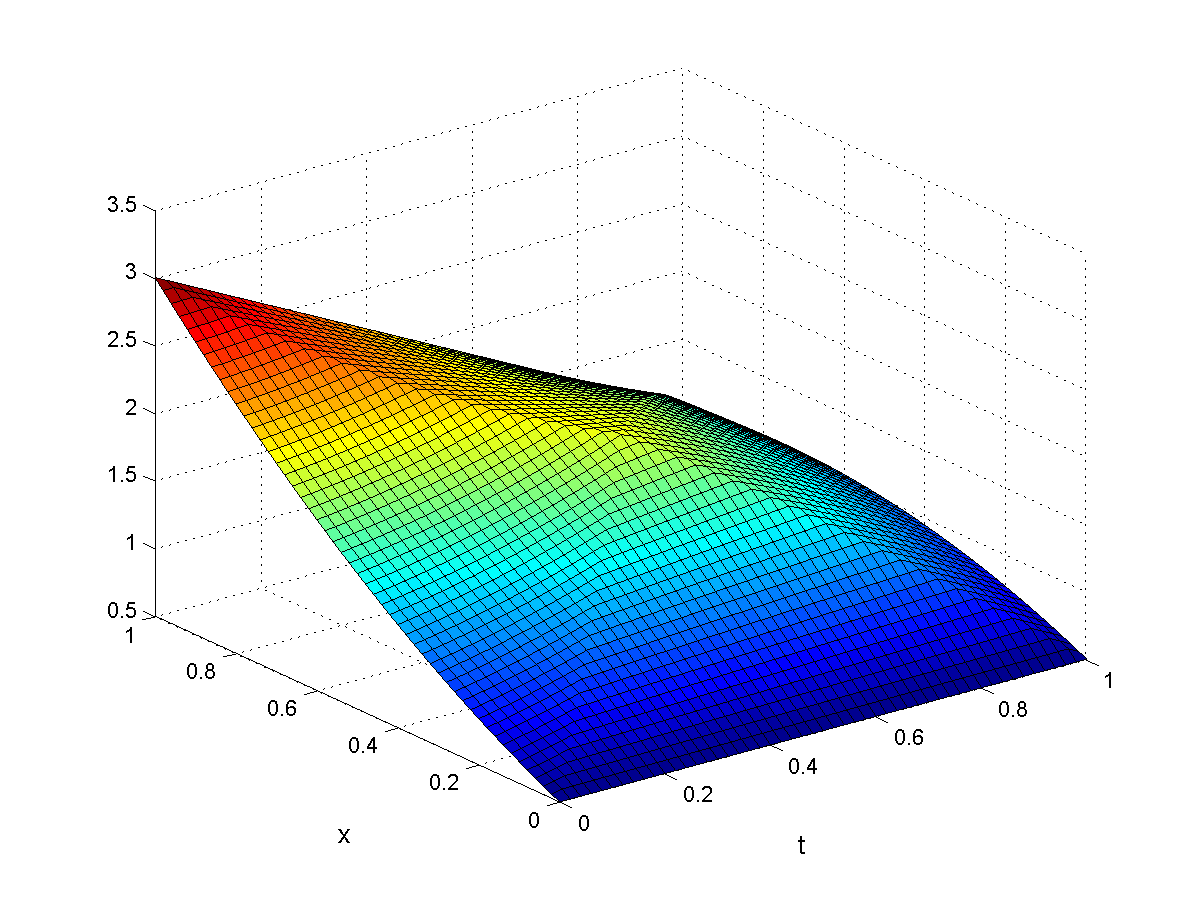
\includegraphics[width = 10cm]{screen.png}
\caption{Колебания струны}
\label{fig:1}	
\end{figure}
\end{document}